\documentclass{scrartcl}
\usepackage[ngerman]{babel}
\usepackage[utf8]{inputenc}
\usepackage[left=1in,right=0.8in,top=0.5in,bottom=0.5in,includeheadfoot]{geometry}
\usepackage[hidelinks]{hyperref}
\usepackage{graphicx}
\usepackage{subcaption}
\usepackage{float}
\usepackage{color}
\usepackage{listings}
\usepackage{dirtree}
\usepackage[autostyle]{csquotes}
\usepackage[backend=biber,style=authoryear,citestyle=authoryear,url]{biblatex}
\bibliography{library.bib}
\lstset{
	language         = Python,
    showstringspaces = false,
    basicstyle       = \small\ttfamily\color{magenta},
    identifierstyle  = \color{black},
    keywordstyle     = \color{red},
    stringstyle      = \color{blue},
    breaklines       = true,
    xleftmargin      = .1\textwidth
}

% add custom product-number field to litarute
\DeclareSourcemap{
    \maps[datatype=bibtex]{
      \map{
        \step[fieldsource=product-number]
        \step[fieldset=usera,origfieldval]
    }
  }
}

\DeclareFieldFormat{usera}{\texttt{#1}}
\AtEveryBibitem{%
    \csappto{blx@bbx@\thefield{entrytype}}{% put at end of entry
        \iffieldundef{usera}{}{\space[Katalog, Artikelnummer: \printfield{usera}]}
    }
}

\renewcommand{\baselinestretch}{1.3}
\renewcommand{\lstlistingname}{Code}
\setlength{\parindent}{0in}
\setlength{\parskip}{1.8ex plus 0.2ex minus 0.3ex}

\title{Texteingabe Vorhersage (next word prediction) für Schwerstmehrfachbehinderte}
\author{Manuel Reich}
\date{April 2015}

\begin{document}

	\maketitle
	\newpage
	
    %table of contents
    \pagenumbering{roman}
    \setcounter{page}{1}
	\tableofcontents
	\newpage

	%content
    \pagenumbering{arabic}
    \setcounter{page}{1}

	\section{Einleitung}
UK erklären
vielleicht next word prediction erklären
\newpage
	\section{Grundlagen}

	\subsection{Eingabegeräte für Schwerstmehrfachbehinderte}
    \label{sec:input-devices}
    
    	Aufgrund der Vielzahl an möglichen Behinderungen und Einschränkungen gibt es eine mindestens genau so große Zahl an Eingabemethoden und Geräten. Diese Eingabegeräte können sowohl eine Schnitstelle zu klassischen PCs darstellen oder auch zur Bedienung von unterstützenden Technologien wie z. B. eines Rollstuhls benutzt werden. Im Folgenden sollen hier exemplarisch einige solcher Eingabegeräte vorgestellt werden. Die hier vorgestellte Auswahl ist nicht vollständig und ist aus den Onlinekatalogen der \emph{RehaMedia GmbH}, und der \emph{REHAVISTA GmbH} sowie den Webseiten der erwähnten Hersteller zusammengetragen.
        
        \subsubsection*{Augensteuerung}
        	Bei der Augensteuerung werden mit Hilfe einer Kamera die Bewegungen der Augen genutzt um ein Gerät zu steuern. Damit können dann auch Windows oder OS X Betriebssysteme mit Hilfe eines On-Screen-Menüs gesteuert werden. Der Anbieter \emph{RehaMedia} bewirbt das System \emph{Tobii PCEye} mit den Worten:" \enquote{Die Augensteuerung erfasst die Augenbewegungen und setzt sie präzise in Mausbewegungen um. Dank eines Mauszeigermenüs stehen auch bei der Bedienung mit der Augensteuerung alle Mausfunktionen wie Doppelklick, Rechtsklick usw. zur Verfügung."} \parencite{rehamedia:TobiiPCEyeGo}
            
         \subsubsection*{Taster}
         	In der Regel handelt es sich bei Tastern um einen einzelnen großen runden Knopf (\autoref{fig:bigRed}). Es gibt aber auch andere Ausführungen wie einen Griff, welchen man zusammendrücken kann oder einen befestigten Stab, gegen den man Druck ausüben kann. Manche Taster können auch an der Kleidung oder an einer Kopfstütze angebracht werden, so dass eine Bedienung nicht nur mit den Händen, sondern auch mit dem Kopf oder durch  Zusammenschlagen der Knie möglich ist. Pedale zur Bedienung mit den Füßen werden auch angeboten. Die meisten Taster verwenden einen 3,5 mm Klinkenstecker und können damit ein einziges Signal (Knopf gedrückt) senden. Der Hersteller \emph{ablenet} bietet z. B. Spielsachen an, die so gesteuert werden können (\autoref{fig:penguinRace}). Andere Eingabegeräte können auch Anschlüsse für diese Taster bereitstellen so dass diese kombiniert werden können.  
         	
            \begin{figure}[H]
				\centering
				\begin{subfigure}{.49\textwidth}
  					\centering
  					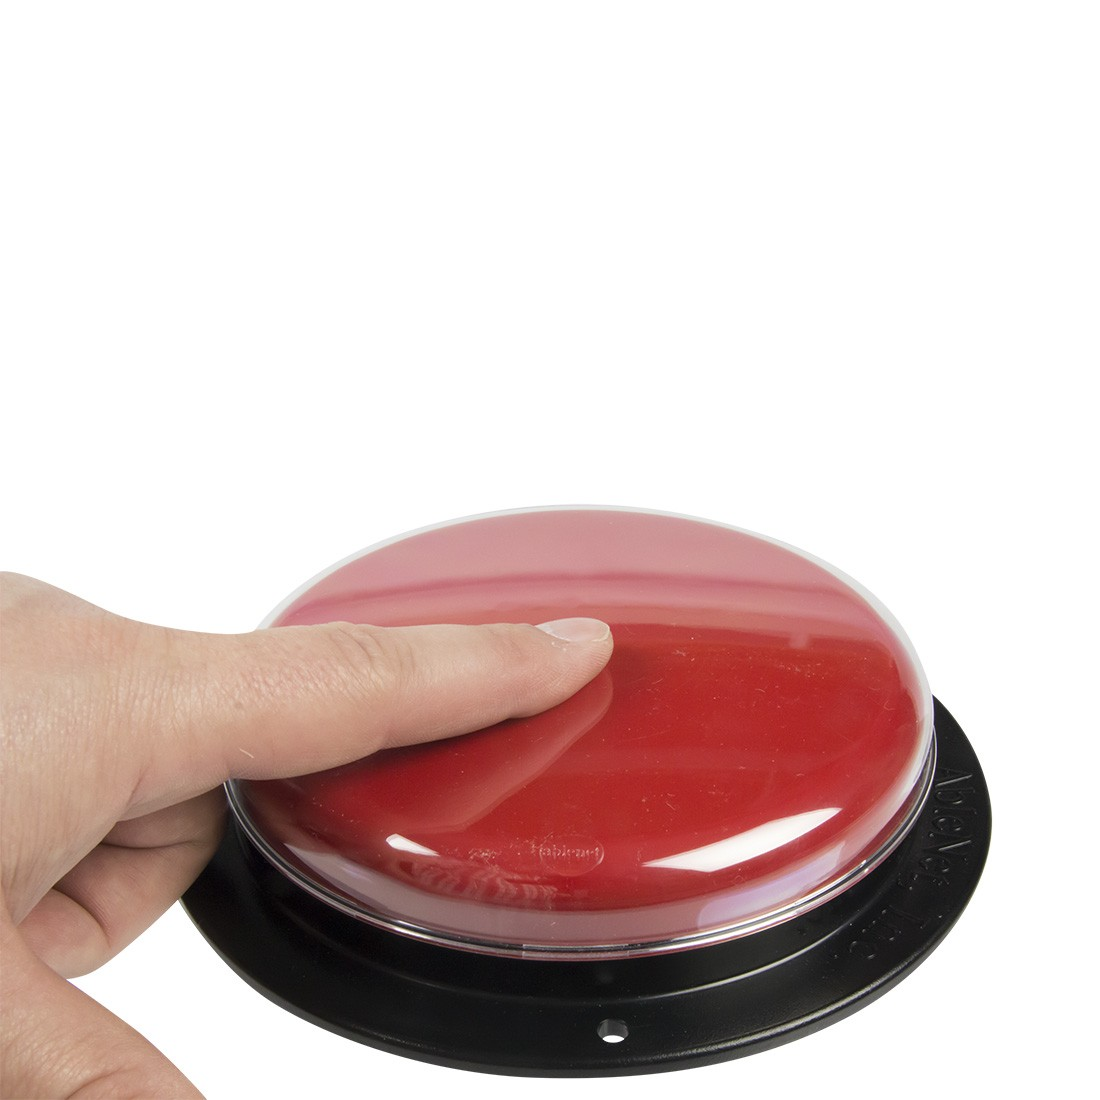
\includegraphics[width=.8\linewidth]{images/big-red-button.jpg}
  					\caption{\emph{Big Red} \cite{ablenet:bigRed}}
                    
  					\label{fig:bigRed}
				\end{subfigure}
				\begin{subfigure}{.49\textwidth}
  					\centering
  					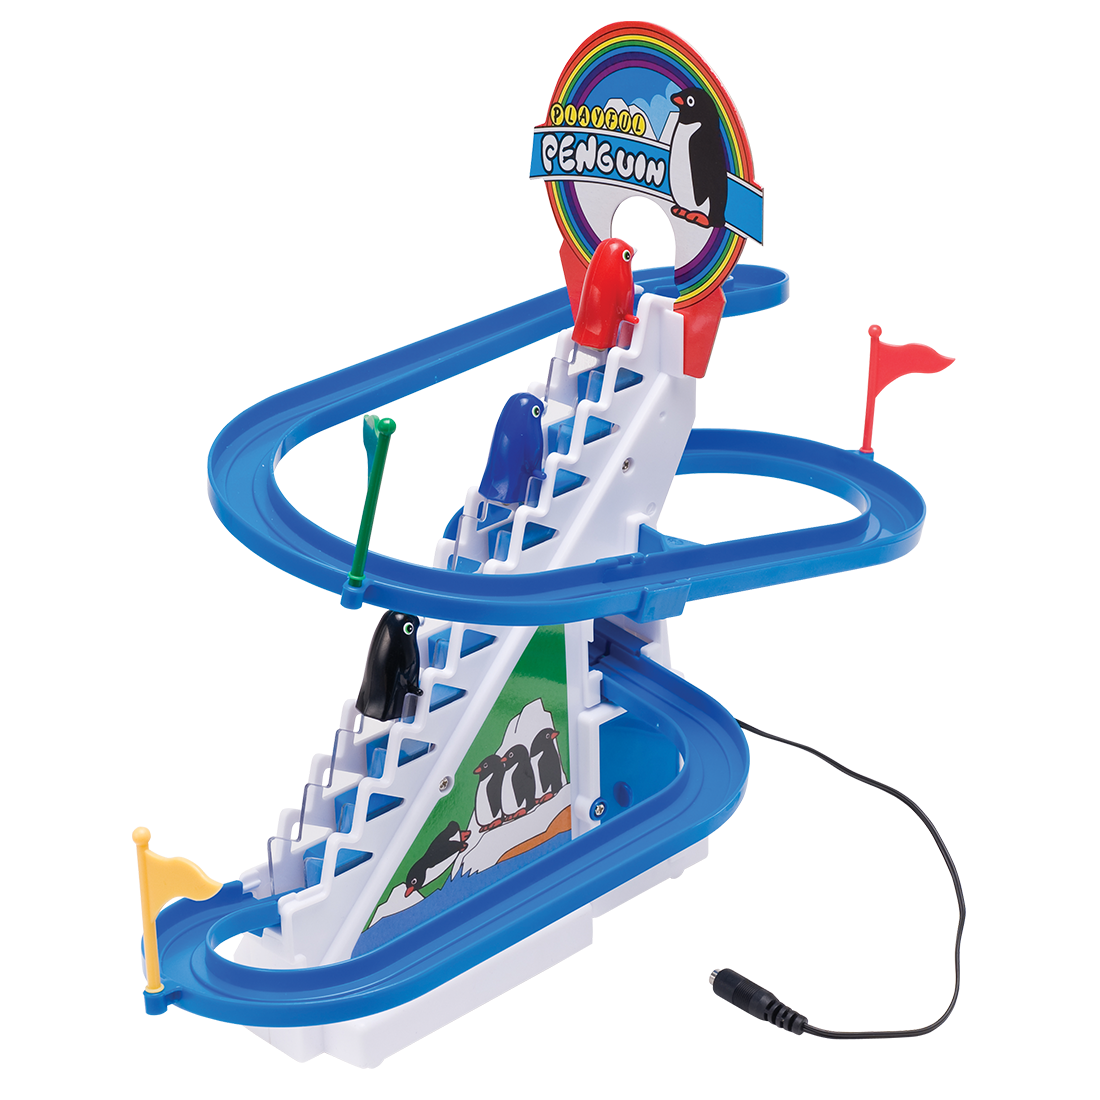
\includegraphics[width=.8\linewidth]{images/penguin-race.png}
  					\caption{\emph{Penguin Race} \cite{ablenet:penguinRace}}
  					\label{fig:penguinRace}
				\end{subfigure}
                \caption{Taster und Spielzeug von ablenet}
				\label{fig:ablenetSingleButtons}
			\end{figure}
            
            Eine weitere Ausführung sind \emph{sprechende Tasten}. Diese Taster haben einen Lautsprecher eingebaut und bieten die Möglichkeit, eine oder mehrere Sprachnachrichten aufzunehmen. Wenn mehrere Nachrichten aufgenommen werden können, kann die auszugebende Nachricht von einer betreuenden Person voreingestellt werden. Andere Geräte funktionieren nach dem Prinzip: einmal drücken gibt Nachricht Nummer eins aus, zweimal drücken Nachricht Nummer zwei und dreimal drücken Nachricht Nummer drei.
            
        	Außerdem gibt es Taster mit mehr als einer Taste. Diese sind dann schon zum Anschluss an Computer oder Tablets gedacht und haben häufig einen \emph{USB}- oder \emph{Bluetooth}- Anschluss. Der Tastenumfang geht dabei von einfachen Geräten mit zwei Tasten bis zu kompletten Computertastaturen.
            
            \begin{figure}[H]
				\centering
				\begin{subfigure}{.33\textwidth}
  					\centering
  					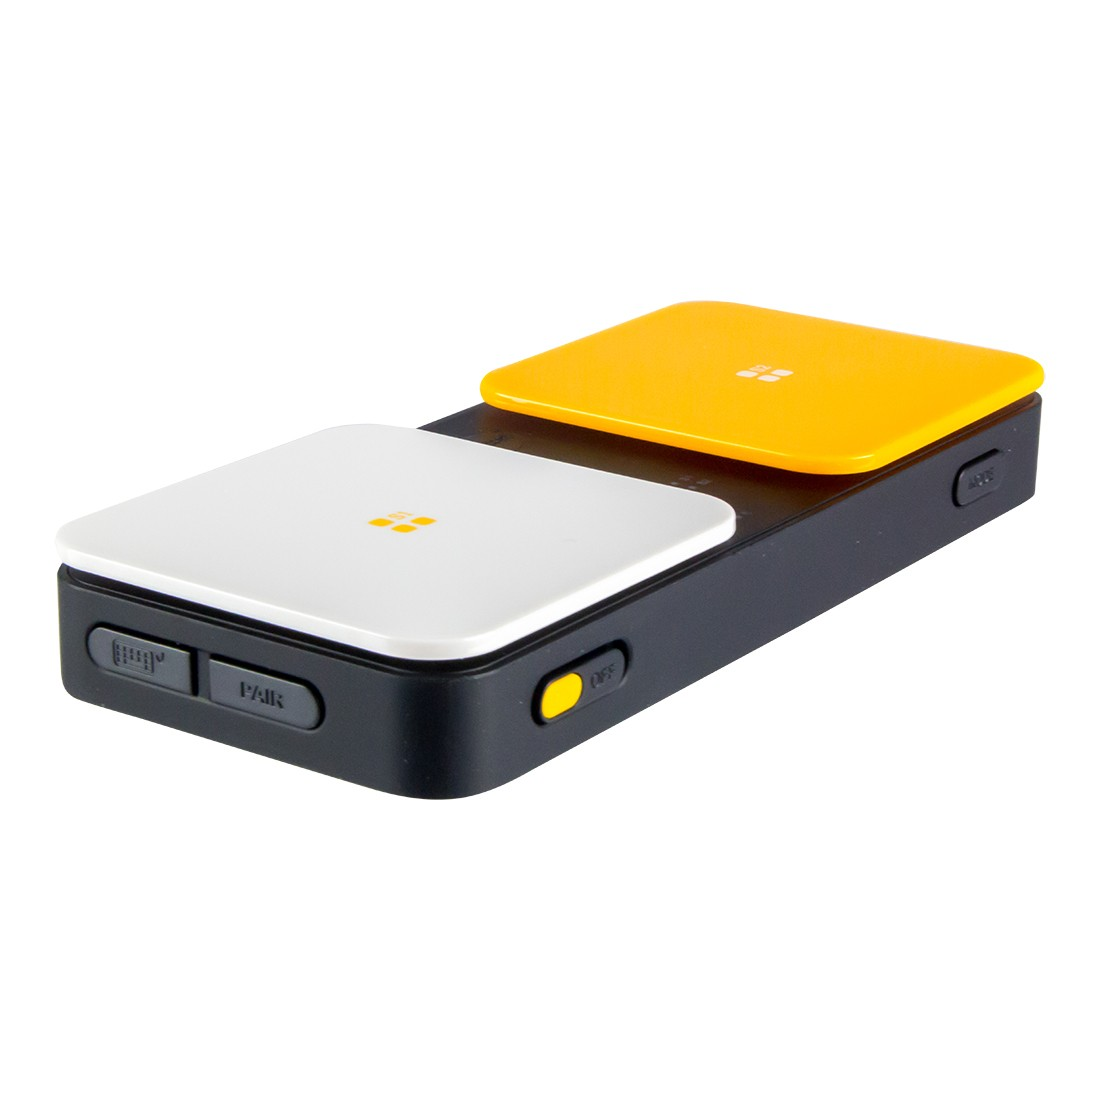
\includegraphics[width=.8\linewidth]{images/buttonsIPad.jpg}
  					\caption{\cite{ablenet:iPad}}
                    
				\end{subfigure}%
				\begin{subfigure}{.33\textwidth}
  					\centering
  					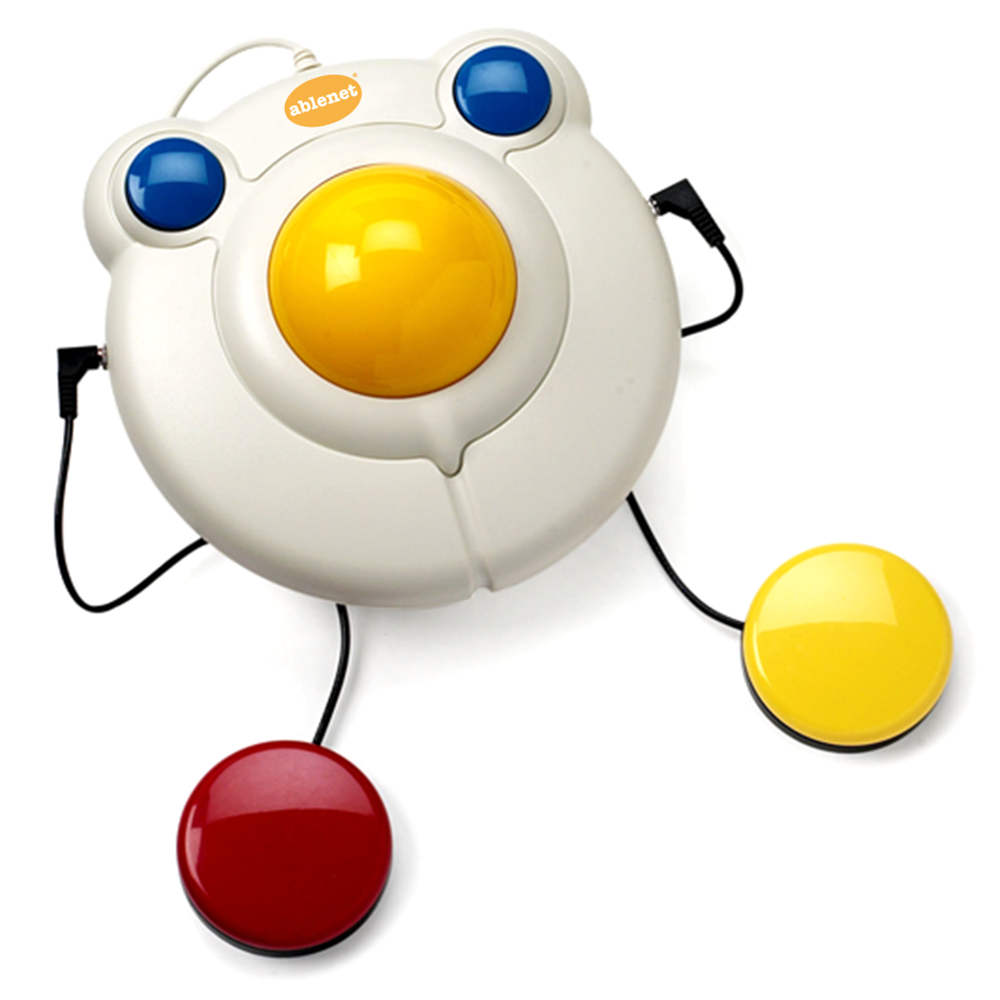
\includegraphics[width=.8\linewidth]{images/buttonsMouse.png}
  					\caption{\cite{ablenet:mouse}}
				\end{subfigure}
                \begin{subfigure}{.33\textwidth}
  					\centering
  					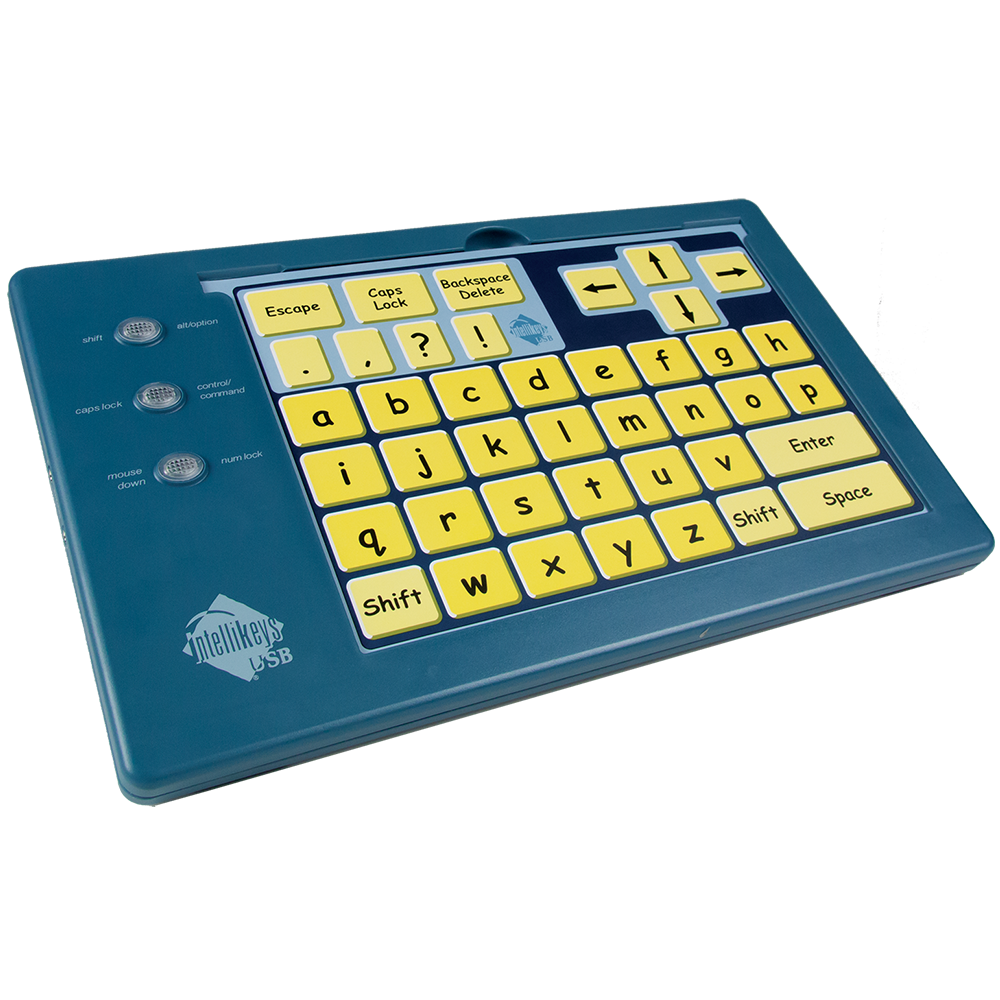
\includegraphics[width=.8\linewidth]{images/buttonsKeyboard.png}
  					\caption{\cite{ablenet:keyboard}}
				\end{subfigure}
                \caption{Taster mit mehreren Tasten von ablenet}
				\label{fig:ablenetMultipleButtons}
			\end{figure}
            
		\subsubsection*{Talker}
        	Bei Talkern handelt es sich um Geräte, mit denen durch Knopfdruck Sprache ausgegeben werden kann. Es existieren sowohl statische als auch dynamische Systeme. Bei statischen Systemen sind die Knöpfe fest in der Hardware eingebaut. Dynamische Systeme verwenden Touchscreens. Oft werden dafür auch handelsübliche Tablets mit Schutzhüllen und Halterungen verwendet. 
            
            Diese Systeme können unterschiedlich komplex sein. Einfachere Talker haben ein festes Set an Symbolen, welche auf Knopfdruck Sprachnachrichten ausgeben. Dynamische Systeme ermöglichen die Navigation durch verschiedene Symbolgruppen oder arbeiten sogar nur mit Text. Manche ermöglichen auch eine Texteingabe per Tastatur. In \autoref{sec:software-examples} werden verschiedene Softwarelösungen für solche Systeme vorgestellt.
            
            \begin{figure}[H]
				\centering
				\begin{subfigure}{.3\textwidth}
  					\centering
  					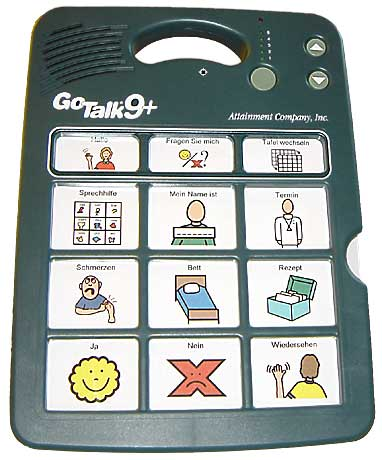
\includegraphics[width=.8\linewidth]{images/goTalkPlus.jpg}
  					\caption{statischer Talker \parencite{rehavista:goTalkPlus}}
                    
				\end{subfigure}
				\begin{subfigure}{.3\textwidth}
  					\centering
  					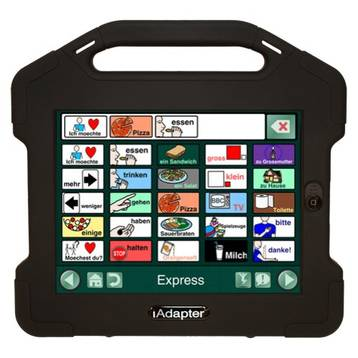
\includegraphics[width=.8\linewidth]{images/goTalkNow.jpg}
  					\caption{iPad mit Talker Erweiterung \parencite{rehamedia:goTalkNow}}
				\end{subfigure}
                \begin{subfigure}{.3\textwidth}
  					\centering
  					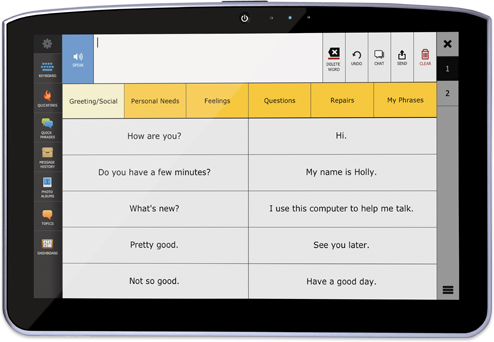
\includegraphics[width=.8\linewidth]{images/tobiiT15.png}
  					\caption{Talker mit literarischem Interface \parencite{tobii:T15}}
                    \label{fig:tobiiT15}
				\end{subfigure}
                \caption{verschiedene Talker}
				\label{fig:talker}
			\end{figure}
            
    \newpage      
    \subsection{Software für Unterstützte Kommunikation}
    \label{sec:software-examples}
    
    	Unter Sprachsoftware wird hier das komplette System von Benutzeroberfläche über mögliche Autovervollständigungen und Eingabevorschlägen bis zur Sprachausgabe verstanden. Im Speziellen soll hier Software vorgestellt werden, die auf den in \autoref{sec:input-devices} beschriebenen \emph{Talkern} Anwendung finden. Die Auswahl der Beispiele richtet sich an ihrer Relevanz für den zu entwickelnden Prototypen. Also Software, deren Funktion den in \autoref{sec:requirements} formulierten Anforderungen nahe kommt.
        
        \subsubsection*{MetaTalkDE / MetaTalkUS}
        	\emph{MetaTalkDE} ist eine iPad App von \emph{Cidar Health Care LLC} für Symbolbasierte \emph{Unterstützte Kommunikation}.
            
            \begin{figure}[H]
				\centering
				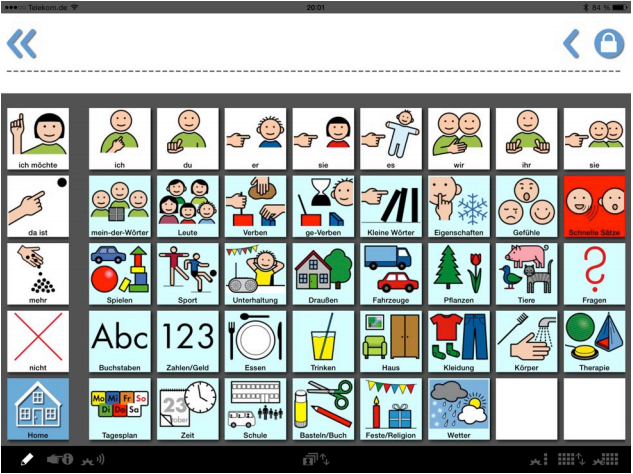
\includegraphics[width=.6\linewidth]{images/Metatalk.png}
                \caption{Schreenshot von MetaTalkDE in der 5x9 Ansicht
                	\parencite[S. 8]{cidar:metaTalkManual}
                }
				\label{fig:metatalk}
			\end{figure}
            
            Auf dem Startbildschirm werden oben in einer Zeile vom Nutzer bereits ausgewählte Symbole angezeigt. Darunter befindet sich ein Raster mit Symbolen und Kategorien. Durch Auswahl einer Kategorie gelangt man auf einen neuen Bildschirm mit entsprechenden Symbolen.
            Durch Druck auf die Symbolzeile oben werden die gelisteten Symbole gesprochen. 
            Laut Handbuch \parencite[S. 7 ff]{cidar:metaTalkManual} ist die Anzahl der Tasten im Raster in drei Stufen (5x9, 4x7, 3x5) anpassbar. Beim Anpassen des Rasters wird auch das Vokabular angepasst. Jede Stufe hat ein eigenes Vokabular, wobei standartmäßig mehr Tasten auch ein größeres Vokabular bedeuten. Die Vokabulare sind innerhalb der App editierbar und können, wie auf Seite 20 f. erklärt, auch über E-Mail ex- und importiert werden. Die gesamte App bietet viele Möglichkeiten der Personalisierung. So können die Symbole der Tasten ausgetauscht werden, neue Tasten hinzugefügt werden, Tasten mit Farben hinterlegt werden und auch Töne für die Sprachausgabe aufgenommen werden (vgl. S.24). Nach Auswahl von Personalpronomen werden die Verben in der passenden Form angezeigt. Dazu lassen sich durch langes Drücken auf ein Symbol andere Formen des entsprechenden Wortes anzeigen. (vgl. S.11 – 14) Auch wird auf Seite 33 erleutert wie sich \emph{Verlinkungen} erstellen lassen, mit denen darauffolgende Symbollisten angezeigt werden.
            
            Da die App auf einem iPad läuft, muss der Nutzer motorisch in der Lage sein, diese mit den Händen zu bedienen. Zwar gibt es die oben beschriebenen \emph{Verlinkungen}, jedoch nutzt die App keine Methoden des \emph{Mashine learning}, um die Eingabe durch optimierte Symbollisten zu erleichtern.
            
        \subsubsection*{Tobii Sono Scribe}
        
        	\emph{Tobii Sono Scribe} ist eine Erweiterung zu der Software \emph{Tobii Communicator}. Die Eingbe ist textbasiert. Das Handbuch \parencite[S. 8]{tobii:sonoScribeManual} beschreibt zwei verschiedene Modi. In einem Modus wird mit einer Liste von vorgeschlagenen Wörtern gearbeitet (\autoref{fig:sonoScribeWords}), in dem anderen wird eine Displaytastatur zur Texteingabe verwendet (\autoref{fig:sonoScribeKeyboard}).
            
            \begin{figure}[H]
				\centering
				\begin{subfigure}{.49\linewidth}
  					\centering
  					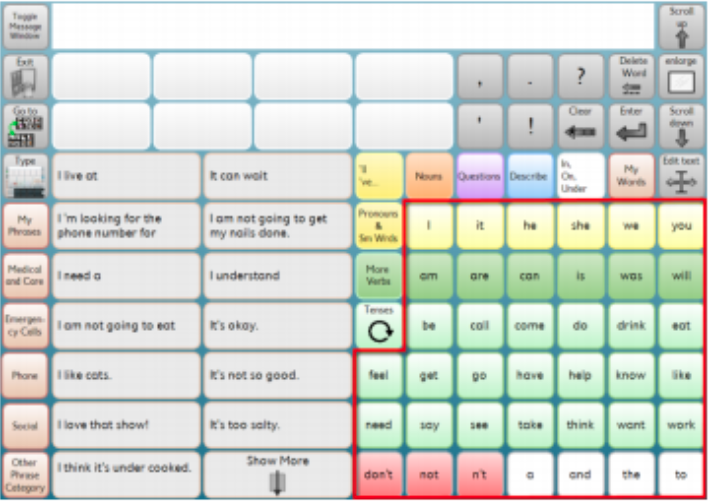
\includegraphics[width=.8\linewidth]{images/sonoScribeWords.png}
  					\caption{Wort Modus 
                    	\parencite[S. 13]{tobii:sonoScribeManual}
                    }
                    \label{fig:sonoScribeWords}
				\end{subfigure}
				\begin{subfigure}{.49\linewidth}
  					\centering
  					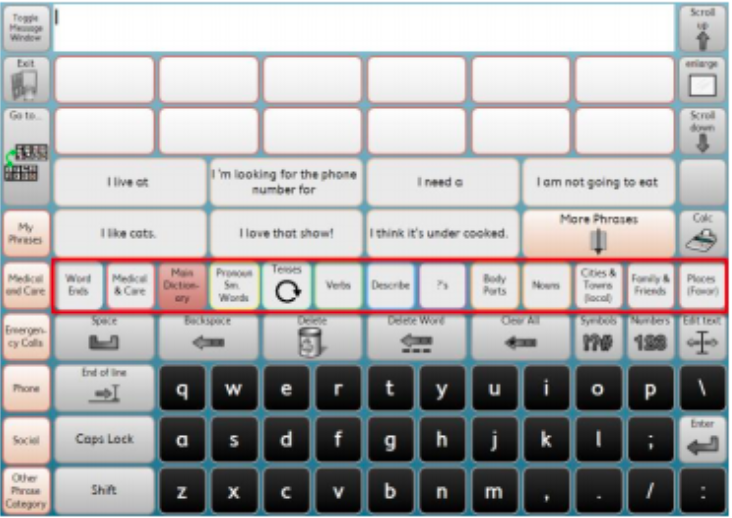
\includegraphics[width=.8\linewidth]{images/SonoScribeKeboard.png}
  					\caption{Tastatur Modus 
                    	\parencite[S. 22]{tobii:sonoScribeManual}
                    }
                    \label{fig:sonoScribeKeyboard}
				\end{subfigure}
                \caption{ }
                \label{fig:sonoScribe}
			\end{figure}
        	
            Die Software kann unter Windows und auf den Geräten von \emph{Tobii} installiert werden. Zum Beispiel auf dem in \autoref{fig:tobiiT15} gezeigtem \emph{T15}. Neben dem enthaltenen Vokabular werden auch verschiedene Listen mit häufig verwendeten Sätzen angeboten, wie auf S. 15 f des Handbuchs beschrieben wird. Sowohl die Sätze, als auch, wie auf S. 20 ergänzt, das Vokabular, sind innerhalb der Software editierbar.
            
            Bei der Eingabe werden wie auf S. 15 beschrieben, mögliche nächste Wörter vorgeschlagen und auch Sätze mit entsprechenden Anfängen aus den gespeicherten Sätzen vorgeschlagen. Im tastaturbasierten Modus werden auch Wortvervollständigungen angeboten (Siehe S. 22). Auf S. 18 wird erklärt, dass Nutzer sich, wie in \autoref{fig:sonoScribeList} zu sehen, auch Listen von Wörtern sortiert nach der Wortart anzeigen lassen können.
            
            \begin{figure}[H]
  				\centering
  				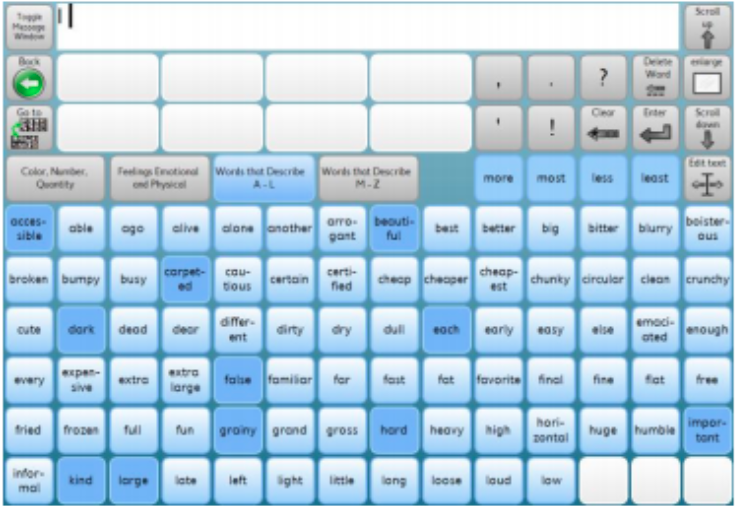
\includegraphics[width=.6\linewidth]{images/SonoScribeList.png}
  				\caption{Liste von Nomen \parencite[S. 18]{tobii:sonoScribeManual}}
                \label{fig:sonoScribeList}
			\end{figure}
            
			Neben der Sprachausgabe gibt es auch einen Texteditor, einen Mailclienten, sowie verschiedene Tools zur Steureung des Windows Betriebssystems. Dazu gehört auch ein PlugIn für den Browser \emph{Mozilla Firefox}. Diese große Anzahl an Funktionen setzt aber voraus, dass Nutzer lesen und schreiben können müssen und fähig sind, die im Vergleich mit \emph{MetaTalkDE} komplexe Benutzeroberfläche bedienen zu können. Die Software unterstützt unter anderem die Eingabe per Touch, Augensteuerung und sogar durch Taster. Bei der Bedienung mit Taster gibt es ein \emph{Scan Raster}, nach dem per Tastendruck von Knopf zu Knopf gesprungen wird.
    
    \newpage
	\subsection{Mashine learning Software für den Massenmarkt}
    \emph{Mashine learning} zur Wortvorhersage wird nicht nur in der \emph{Unterstützten Kommunikation} angewendet, sondern auch in der Software für den Massenmarkt. Im Folgenden sollen hier kurz drei Beispiele vorgestellt werden, die Nutzern Worte zur Eingabe vorschlagen.
        
        \subsubsection*{swiftKey}
        	In einem Artikel für die Webseite \emph{techrepublic.com} beschreibt \cite{techrepublic:swiftKey} die Funktionen der Bildschirmtastatur für mobile Geräte \emph{swiftKey}. Zuerst erwähnt er, wie Nutzern dank eines lernfähigen Algorythmus Worte vorgeschlagen werden. Im optimalen Fall müsste man also nach Eingabe des ersten Wortes gar nicht mehr tippen. Dann beschreibt er die zweite Funktion, welche \emph{Flow} genannt wird. Hierbei wird zum Tippen nicht abgesetzt, sondern mit dem Finger von einem Buchstaben zum anderen gewischt. Die Tastatur kann auch so das gewünschte Wort erkennen.
        
        
        \subsubsection*{iOS QuickType}
        
        	Die Bildschirmtastatur für \emph{Apple iOS 8} enthält ein Feature mit dem Namen \emph{QuickType}. Die Funktion ist ähnlich zu \emph{swiftKey}. Auch hier werden beim Tippen Worte vorgeschlagen. \emph{Apple} bewirbt auf seiner Webseite, dass die Wortvorschläge Kontextabhängig sind. So wird beschrieben, dass in einem Mailprogramm andere Worte vorgeschlagen werden, als in einem Chat mit einem Freund. Außerdem kann die Tastatur laut \cite{apple:quickType} auch einen eingehenden Text in einer Chatapplikation analysieren und entsprechende Vorschläge für die Antwort machen. Eine Funktion zum Tippen ohne abzusetzen gibt es nicht.
        
        \subsubsection*{Google Suggest}
        
        	Auch \emph{Google} schlägt Nutzern Worte vor, während diese Begriffe in die Suchmaschine eingeben. Dieser Service nennt sich \emph{Google Suggest}. Dies beschreibt \cite{google:suggestIntro} im offiziellen Blog von Google. Außerdem erwähnt sie, dass der Service auch Rechtschreibfehler verbessern kann. In einem anderen Blogeintrag erklärt \cite{google:suggestUpdate}, dass \emph{Goggle} 2\% die eingegeben Suchanfragen zusammen mit der IP-Adresse des Nutzers auswertet und aus diesen Daten die Vorschläge generiert.
    
    
    
    \newpage
	\section{Anforderungen}
    
	\subsection{Eingabe}
    	Ziel dieser Arbeit ist die Entwicklung eines Prototypen einer Sprachapplikation. Mit dieser Applikation soll ein stummer und motorisch eingeschränkter Nutzer Sätze erzeugen können, die per Sprachausgabe ausgegeben werden können. Dabei soll es nicht nötig sein zu tippen. Sätze werden erzeugt indem ein Wort nach dem anderen aus einer Liste von Wörtern ausgewählt wird. Am Ende wird der Satz bestätigt und ausgegeben. Sollte ein Wort ausversehen zum Satz hinzugefügt worden sein soll es möglich sein diesen Fehler zu korrigieren und das Wort wider aus dem Satz zu entfernen. Das erste Wort in der Liste ist dabei das Wort welches am wahrscheinlichsten als nächstes im aktuellen Satz vorkommen wird. Alle weiteren Wörter sind dann nach absteigender Wahrscheinlichkeit sortiert.
         
    	Dieses Kapitel befasst sich mit den Anforderungen bezüglich der Eingabe die sich an die Applikation stellen. Aufgrund der Vielzahl an möglichen Behinderungen und Einschränkungen gibt es eine mindestens genau so große Zahl an Eingabemethoden und Geräten. In vielen Fällen sind Eingabegerät und Software eng miteinander verbunden oder sogar ein in sich abgeschlossenes System.
        
        Um möglichst viele verschiedene Eingabegeräte zu unterstützen soll die zu entwickelnde Applikation nicht direkt auf spezielle Geräte angepasst werden. Darum werden hier nicht bestimmte Aktionen zur Eingabe beschrieben sondern Signale welche dann von verschieden Geräten erzeugt werden können. Ein Signal kann jeder diskreter Code sein der von einem Eingabegerät an die Software gesendet werden kann. Beispielsweise das Drücken einer bestimmten Taste auf einer Tastatur. Für die Entwicklung des Prototypen sollen Signale dann auch über die Tastatur erzeugt werden. Es ist auch denkbar komplizierte Eingabemethoden zu implementieren um die tatsächliche Nutzerfreundlichkeit besser darzusetllen. Schließlich ist das Tippen einer Taste doch sehr viel einfacher als z. B. das Betätigen eines Kopfschalters an einem Rollstuhl. 
        
        Da nicht jedes Eingabegerät die gleiche Anzahl an Signalen liefert soll hier ein Minimum von drei diskreten Signalen festgelegt werden. Mit diesen drei Signalen sollen alle Funktionen der Applikation umzusetzen sein. Dabei ist es möglich, dass das gleiche Signal in einem anderen Kontext eine andere Bedeutung hat. Es ist auch vorstellbar, wenn unbedingt nötig, eine weitere Funktion durch Wiederholen des gleichen Signals innerhalb eines gewissen Zeitraums aufzurufen. Diese Einschränkung wäre natürlich für Nutzer von Eingabegeräten welche mehr als drei Signale erzeugen können schnell frustrierend. So soll es möglich sein auf weitere Signale zu reagieren und mit diesen Erleichterungen in der Bedienung der Applikation umzusetzen. Ein Beispiel hierfür wäre eine Liste, die sich über mehrere Zeilen erstreckt. Es ist möglich durch diese mit einem einzigen "weiter" Befehl zu navigieren. Wenn möglich wäre es aber auch wünschenswert eine Zeile nach unten oder eben auch zurück zu navigieren.
        
        Bei der Betrachtung bestehender Eingabegeräte fallen weitere Anforderungen an die Bedienung der Applikation auf. Es gibt verschiedene Eingabegeräte die zur Steuerung eines Mauszeigers gedacht sind. Meist scheint hier die Bedienung der Maus etwas komplizierter als mit einer klassischen Computermaus. Andere Geräte arbeiten mit verschieden angeordneten großen Tasten, manche bilden diese Tasten auch auf einem Touchscreen ab. Darum sollte es auch möglich sein die Schaltflächen der Applikation klassisch per Maus oder Fingerdruck auswählen zu können. Dabei sollte auf die ungewöhnliche Steuerung des Mauszeigers oder motorische Einschränkungen bei der Bedienung von Touchscreens Rücksicht genommen werden.
        
        Ziel dieser Abstrahierung der Eingabehandhabung ist zum einen die Konzentration der Arbeit und des Prototypen auf die Sprachanalyse und die Visualisierung der Ergebnisse. Zum Anderen aber auch der Versuch die Grundlagen für ein Modulares System zu skizzieren welches auch mit zukünftigen noch nicht existierenden Eingabegeräten funktionieren kann. Ein Beispiel hierfür wäre der bereits erwähnte Mauszeiger der eben nicht nur über eine klassische Maus gesteuert werden kann sondern unter anderem auch mit Trackpad, Trackball oder Trackpoint.
        \newpage
        
        
        
	\subsection{Kathegorie-auswahl / -erkennung}
    	Da zur Prädiktion von wahrscheinlichen nächsten Wörtern zuerst einmal ein Satzanfang benötigt wird startet man zu Beginn mit einer Kategorieübersicht. Hier sollen die Kategorien auch als Liste dargestellt werden. Basierend auf der Kategorieauswahl soll nun eine Liste von möglichen Satzanfängen oder möglichen ersten Wörtern eines Satzes angezeigt werden. 
        
        Durch die enorme Einschränkung der möglichen Eingabesignale kann das navigieren durch lange Listen sehr zeitaufwändig werden. Natürlich stehen im optimalen Fall die benötigten Wörter am Anfang der Liste. Es ist aber zu erwarten, dass es immer wieder Fälle gibt bei denen keine sinnvolle oder hilfreiche Prädiktion gemacht werden kann. Um in diesem Fall immer noch eine einigermaßen überschaubare und sinnvolle Liste erstellen zu können, soll der Wortschatz der Kategorie entsprechend eingeschränkt werden. Dabei ist es denkbar mit Unterkategorien zu arbeiten welche automatisch aufgrund der Vorherigen Sätze bestimmt werden. Diese Unterkategorisierung soll im Hintergrund vom Nutzer unbemerkt stattfinden.
        
        Oberkategorien dagegen werden vom Nutzer bewusst und manuell ausgewählt. Auch soll es zu jeder Zeit möglich sein die bestehende Oberkategorien zu wechseln um somit Zugang zu einem anderen Wortschatz zu erhalten.
        
        -> irgendwas zur Bestimmung von Kategorien
        \newpage
        
        
       	\subsection{Ausgabe}
        
        -> Oben Satz unten Wörter
        -> sehr reduziertes interface
        -> Nach auswahl eines Worts wird neue Liste generiert
        -> Liste als raster von buttons
        -> color coding von Wortarten?
        -> konjugierung nach Eigabe ?
        -> sprachausgabe nicht teil der Arbeit da trivial
        -> Applikation in englischer Sprache
        -> skalierbar aber konzipiert für typische tablets
           also c.a. DinA4
        -> "zurück Button" zur Kategorieauswahl auf Listeposition -1
        -> max 70 Wörter -> alles darüber zu Zeitaufwändig schnelle  
           Bedienug über kompletter Wortschatz
    
    
    
    
    
    
    
    
    
    
    
    
    
    
    
    
    
    
    
    
	\section{NLP}

\subsection{Klassifizierung}
\subsection{next word prediction}
  \subsubsection{Language models}
  \subsubsection{corpora and Statistiken}
  \subsubsection{Bibliotheken und APIs}
    
	\section{Design}
	
    In diesem Abschnitt wird der Aufbau des Prototypen erklärt Und die darin verwendeten Technologien vorgestellt. Mann kann den Prototypen in drei wesentliche Teile gliedern.
            
	\begin{description}
		\item[Das Framework] ist vor allem für die Benutzeroberfläche und für das Verarbeiten von Benutzereingaben verantwortlich. Es dient als Rahmen der Applikation und ist für die kommunikation mit dem jeweiligen Betriebssystem zuständig.
        
        \item[Learner und Predictor] sind für den \emph{Natural Language Processing} Teil der Anwendung zuständig. Der \emph{Learner} kann neue Sprachmodelle aus Texten erzeugen. Der \emph{Predictor} kann mit diesen Sprachmodellen Wortlisten liefern. 
        
        \item[Adapter] bilden Signale von verschiedenen Eingabegeräten auf die vom Prototypen definierten Signale ab. Sie ermöglichen es \emph{Plugins} für weitere Eingabegeräte zu schreiben.
	\end{description}
    
	\subsection{Das Framework}
    	Die Software ist in \emph{Python} geschrieben. \emph{Python} scheint eine viel für \emph{Natural Language Processing} verwendete Sprache zu sein. Sucht man z. B. auf \emph{github.com} nach den in \autoref{tab:githubNLP} gezeigten Begriffen, liegt Python als Sprache immer weit vorne.
        
        \begin{figure}[H]
			\centering
                
			\begin{tabular}{ r || c | c | c}
                \diagbox{Sprache}{Suchbegriff} & NLP & Natural Language & Natural Language Processing \\ \hline \hline
                Python & 1168 & 500 & 348\\ \hline
                Java & 740 & 269 & 172\\ \hline
                JavaScript & 135 & 146 & 37 \\ \hline
                Ruby & 103 & 100 & 28 \\ \hline
                C++ & 76  & 45 & 23 \\ \hline
            \end{tabular}
            \caption{Anzahl gefundener Repositories in den top fünf Sprachen auf \texttt{https://github.com/search} (besucht am 02.07.2015)}
			\label{tab:githubNLP}
		\end{figure}
        
        Für die Benutzeroberfläche wird ein \emph{open source framework} mit dem Namen \emph{Kivy} verwendet. Laut der Offiziellen Webseite \parencite{kivy:homepage} laufen mit \emph{Kivy} geschriebene Aplikationen unter Linux, Windows, OS X, Android und iOS. Dazu muss die Applikation für jedes entsprechnende System gepackt werden.
        
        In der \texttt{main.py} Datei wird die \texttt{run} Funktion von \emph{Kivy} aufgerufen. Diese startet die Applikation, setzt \emph{listener} auf die verfügbaren \emph{Adapter} und instanziiert einen \emph{Predictor}.
        
	\subsection{Learner und Predictor}
    
    	Der \emph{Learner} besteht aus zwei speraten Teilen. Sus einem \emph{Tokenizer} und einem \emph{Clusterer}. Der \emph{Tokenizer} hat die Aufgabe, Texte wie sie z.B. in einem Buch zu finden sind, zu bereinigen. Dem \emph{Tokenizer} werden mehrere Textdateien übergeben aus welcher dieser eine einzelne neue Textdatei generiert. Darin befindet sich der bereinigte Text in einer Form wie er von dem \emph{Clusterer} gelesen werden kann.

		Der \emph{Clusterer} liest und analysiert die vom \emph{Tokenizer} generierte Textdatei. Dieser Umweg über eine extra generierte Datei ist nötig, da für den \emph{Clusterer} eine \emph{third party} Lösung verwendet wird. Dies wird in \autoref{sec:thirdTry} genauer beschrieben. In erster Linie gruppiert der \emph{Clusterer} die übergebenen Worte in Klassen und speichert das Ergebniss wieder in mehreren Dateien ab. Die vom \emph{Clusterer} generierten Dateien werden im folgenden \emph{Sprachmodell} genannt.

		Das generieren von \emph{Sprachmodellen} ist nicht Teil der gepackten Applikation. Dazu muss für jedes neue Sprachmodell der \emph{Tokenizer} und der \emph{Clusterer} von Hand aufgerufen werden. Das generierte \emph{Sprachmodell} wird dann in den dafür vorgesehen Ordner in der Applikation gelegt.

		In der laufenden Applikation kann der Nutzer eine Kategorie auswählen. Diese entspricht immer einem \emph{Sprachmodell}. Nach der Auswahl wird wird dieses automatisch von dem \emph{Predictor} geladen. Dieser Prozess wird in \autoref{sec:implemetation-wordPredition} genauer beschrieben. Aufgrund des Sprachmodells wird vom \emph{Predictor} dann eine Wortliste generiert.
        
    \subsection{Adapter}
    
    	Ein \emph{Adapter} besteht aus einer einzigen \emph{Python} Datei mit dem Namen des Gerätes kombiniert mit dem Wort \emph{Adapter}. Jeder \emph{Adapter} muss von der Klasse \texttt{SuperAdaper} erben.

		Jeder neue \emph{Adapter} muss in dem Ordner \texttt{inputAdapters} gespeichert werden. Auserdem muss dieser in der \texttt{\_\_init\_\_.py} im gleichen Ordner importiert und in die Liste \texttt{adapters} eingetragen werden. Durch diesen Prozess wird erreicht, dass für das Hinzufügen von einem \emph{Adapter} nur Änderungen innerhalb eines einzigen Ordners vorgenommen werden müssen.

		\texttt{SuperAdaper} wiederum erbt von \emph{Kivy}'s \texttt{EventDispatcher}.
So ist es einfach innerhalb der Applikation auf Signale zu reagieren.
Singnale sind einfache Strings bestehend aus dem kleingeschribenen Namen des Signals. Ein \emph{Adapter} muss eine statische Funktion \texttt{is\_available()} implementieren, die angibt ob das zum \emph{Adapter} entsprechnde Gerät verfügbar ist. Sollte das nicht der Fall sein wird ein \emph{Adapter} nicht geladen.

		Des weiteren muss ein \emph{Adapter} minnimal die drei Signale \texttt{left}, \texttt{right} und \texttt{enter} senden können. Wenn möglich kann ein Adapter auch noch weitere Signale senden. Mögliche weitere Signale sind: \texttt{up}, \texttt{down}, \texttt{talk} und \texttt{close}.
        
	
    \newpage	
	\section{Implementierung}
    \subsection{User Interface}
    
    	Zur Installation von \emph{kivy} unter Mac OS X wird auf der offiziellen Seite eine gepackte .app Datei angeboten. Wenn man sich diese genauer ansieht, enthält diese eine eigene \emph{Python}-Installation inklusive aller von \emph{kivy} benötigten Pakete. Allerdings kann man so seine \emph{Python}-Dateien nur mit dieser \emph{kivy App} ausführen. Ein versprochenes Shellscript, welches zumindest einen \texttt{kivy} Befehl für die Komandozeile bereitstellen soll, fehlt im Downloadverzeichnis. Es war auch nicht möglich diese Funktion von Hand mithilfe von Symlinks herzustellen.
        
        Auch abgesehen von diesen Problemen wäre es wünschenswert, \emph{kivy} in einer eigenen virtuellen \emph{Python}-Umgebung, erstellt von \texttt{virtualenv} über den Paketmanager \texttt{pip} zu installieren. Auf diese Weise können weitere für die Applikation benötigten Pakete auch in dieser Umgebung installiert werden.
        
        Das \emph{kivy} Framework bietet neben einem Eventsystem vor allem eine große Sammlung an User Interface Elementen und Layouts. Diese sind normale \emph{Python}-Klassen und können im Code instanziiert werden. Allerdings bietet \emph{kivy} auch eine eigene Syntax namens \emph{kv} (oder kivy-language) an, mithilfe welcher man die Layouts deskriptiv erstellen kann. Die Sprache erinnert ein wenig an eine Mischung aus dem \emph{CSS} Preprocessor \emph{Sass} und der \emph{HTML} Template Sprache \emph{Haml}.      
        
        \begin{figure}[H]
    		\centering
    		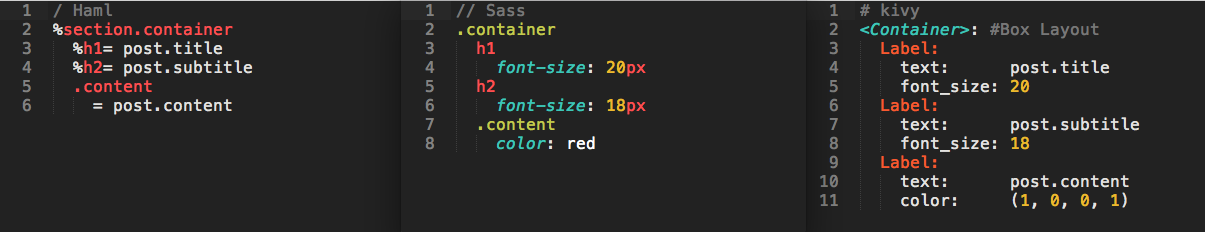
\includegraphics[width=15cm]{images/hamlsasskv.png}
    		\caption{Vergleich zwischen Haml Sass und kv}
    		\label{img:HamlSassKv}
		\end{figure}
        
        Man kann in \emph{kv} zwar auf \emph{Python}-Ausdrücke und Variablen zugreifen, aber alle Arten von Kontrollfluss  – wie z. B. Schleifen – stehen nicht zur Verfügung. So kann eine Liste von Buttons mit der Länge aller gefundenen Wortvorschläge nicht allein in \emph{kv} beschrieben werden. Als Lösung hierfür wurde in dieser Arbeit die Oberfläche in einzelne Module zerlegt. Jedes Modul hat eine eigene Klasse und dazu eine eigene \emph{kv} Datei. Die \emph{Python}-Klasse übernimmt so die Aufgabe eines Controllers, während die \emph{kv} Datei den View beschreibt. Allerdings werden immer noch viele Teile des Views im Controller instanziiert.
        
	\newpage
    \subsection{Wortschatz Verwaltung}
	\subsection{Kathegorisierung}
	\subsection{Wortvorhersage}
    \newpage
	\section{Ergebniss}
	\section{Resuemee}



    
    \printbibliography




\end{document}